\renewcommand{\appendixname}{Anexo}
\renewcommand{\thechapter}{\Alph{chapter}}

% Comando para iniciar la sección de anexos en el índice
\newcommand{\initappendix}{%
  \addcontentsline{toc}{chapter}{Anexo}%
}

% Comando para cada anexo individual
\newcommand{\anexo}[1]{%
  \refstepcounter{chapter}%
  \chapter*{Anexo \thechapter: #1}%
  \addcontentsline{toc}{section}{Anexo \thechapter: #1}%
  \markboth{Anexo \thechapter: #1}{}%
}

\initappendix

\anexo{Cronograma de Actividades}

En líneas generales, el desarrollo del proyecto avanzó conforme a lo planificado. No obstante, se registró una demora puntual en la implementación del asistente conversacional (chatbot), principalmente asociada a la integración segura con el servicio de autenticación (uso de \textit{tokens} de sesión), el rediseño de la API interna (\texttt{/api/chat}) y el manejo robusto de estados de error y límites de servicio (cuotas, \textit{timeouts} y cancelación de respuestas).

Como medidas de mitigación se replanificaron iteraciones, se paralelizaron tareas no críticas (predicción y dashboard) y se incorporaron pruebas de usabilidad y validaciones adicionales en la IU (historial, selector/archivo de conversaciones y retroalimentación de errores). Esta reprogramación desplazó parcialmente el hito del chatbot sin modificar el alcance funcional comprometido ni afectar los entregables finales del trabajo.

A continuación, se presenta el cronograma actualizado con las tareas realizadas, en curso y reprogramadas, que reflejan el estado actual del proyecto.

\begin{figure}[ht]
    \centering
    \includegraphics[width=0.7\textheight]{./././images/Cronograma.png}
    \caption{Cronograma de actividades.}
\end{figure} % En las entregas que no son la entrega final, se debe tener al menos un anexo con el cronograma (Gantt)
\anexo{Resultados de la encuesta}

% --- Parte 1
\begin{figure}[htbp]
  \centering
  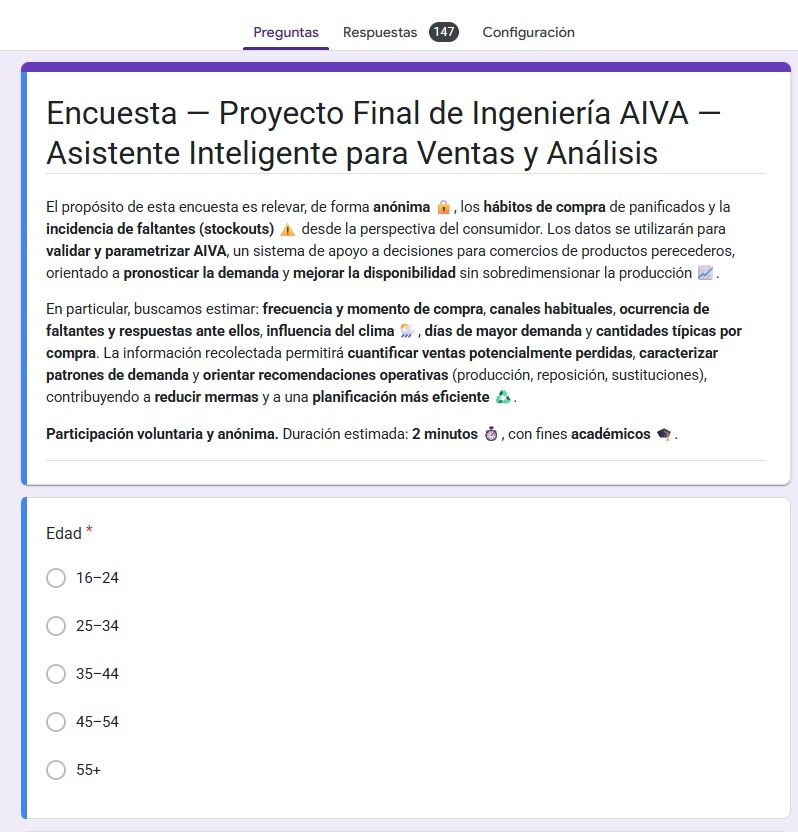
\includegraphics[width=0.92\textwidth]{images/encuesta_p1.png}
  \caption{Encuesta “Proyecto Final de Ingeniería AIVA” — parte 1}
  \label{fig:encuesta-aiva-1}
\end{figure}

% --- Parte 2
\begin{figure}[htbp]
  \centering
  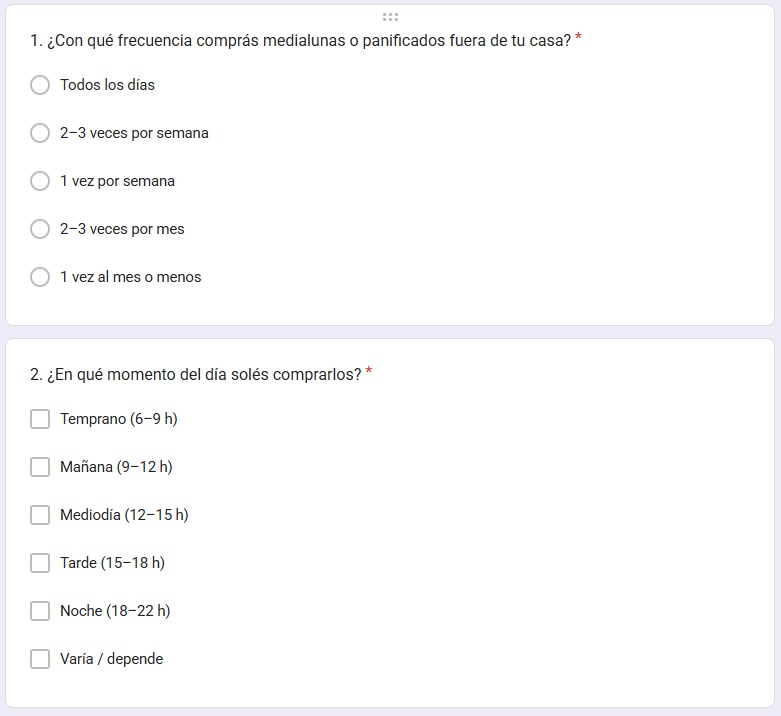
\includegraphics[width=0.92\textwidth]{images/encuesta_p2.png}
  \caption{Encuesta “Proyecto Final de Ingeniería AIVA” — parte 2}
  \label{fig:encuesta-aiva-2}
\end{figure}

\begin{figure}[htbp]
  \centering
  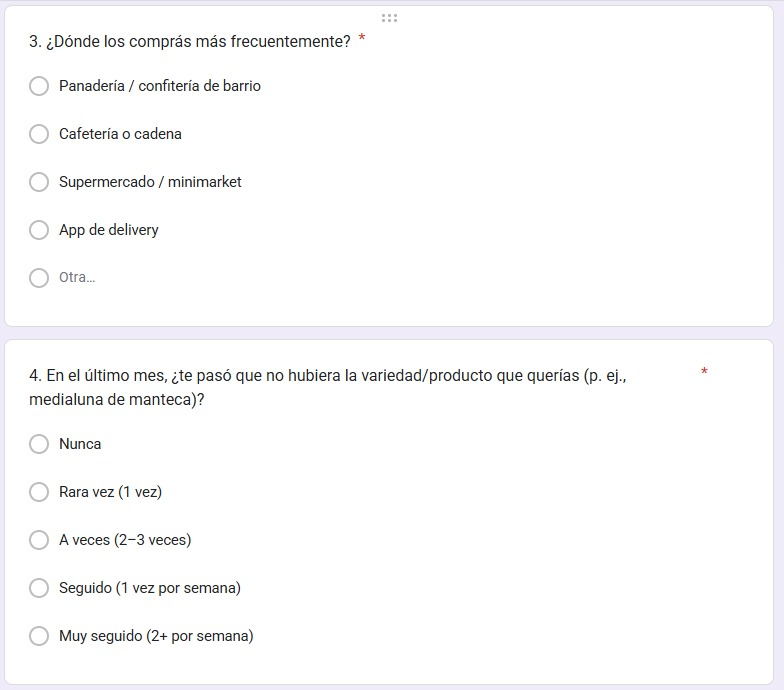
\includegraphics[width=0.92\textwidth]{images/encuesta_p3.png}
  \caption{Encuesta “Proyecto Final de Ingeniería AIVA” — parte 3}
  \label{fig:encuesta-aiva-3}
\end{figure}

\begin{figure}[htbp]
  \centering
  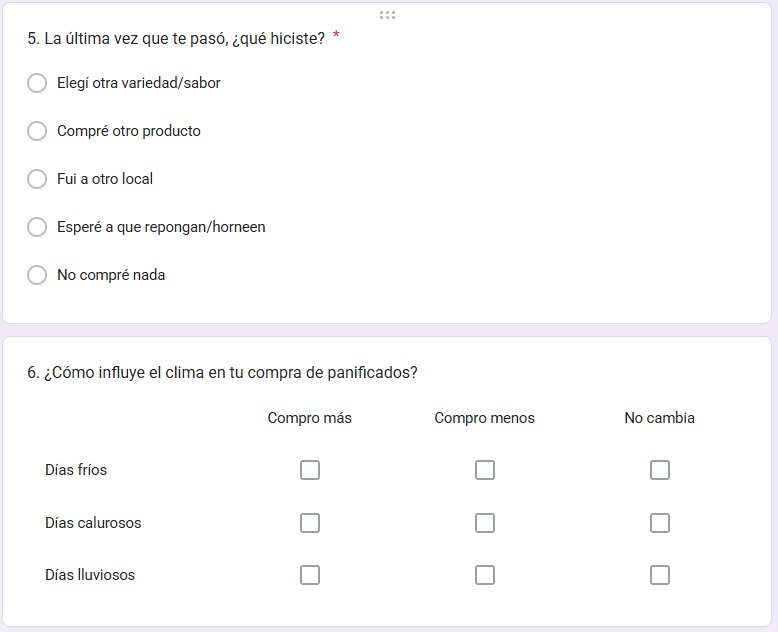
\includegraphics[width=0.92\textwidth]{images/encuesta_p4.png}
  \caption{Encuesta “Proyecto Final de Ingeniería AIVA” — parte 4}
  \label{fig:encuesta-aiva-4}
\end{figure}


\begin{figure}[htbp]
  \centering
  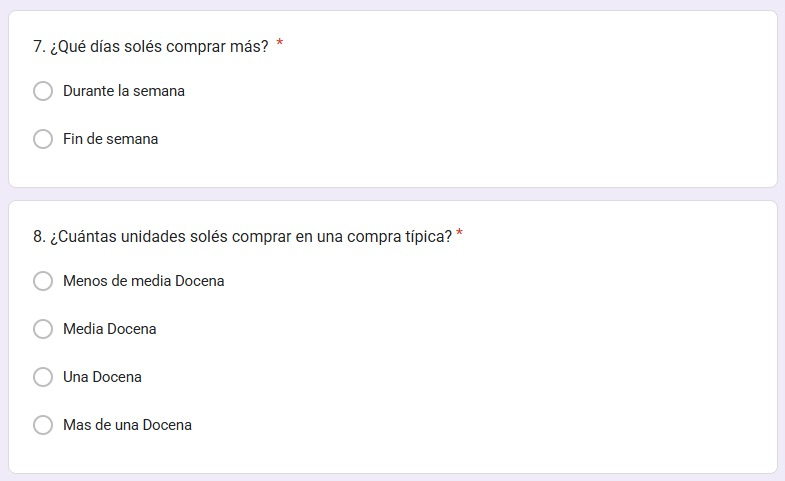
\includegraphics[width=0.92\textwidth]{images/encuesta_p5.png}
  \caption{Encuesta “Proyecto Final de Ingeniería AIVA” — parte 5}
  \label{fig:encuesta-aiva-5}
\end{figure}
\clearpage

 % En el caso de tener en cuestas tiene que haber una transcripción de los resultados
\anexo{Transcripción de entrevista a Milena de La Catalana}

\textbf{Entrevistador:} Para comenzar, ¿podrías contarnos tu nombre, el nombre del negocio y hace cuánto tiempo están trabajando?  

\textbf{Milena:} Mi nombre es Milena González. Trabajo en la confitería La Catalana, que es un negocio familiar que está en funcionamiento hace aproximadamente 15 años.  

\vspace{0.5em}

\textbf{Entrevistador:} ¿Cuántos empleados tiene su negocio?  

\textbf{Milena:} El negocio tiene 19 empleados.  

\vspace{0.5em}

\textbf{Entrevistador:} ¿Cuáles son los productos más y menos vendidos, y cuánto tiempo duran en promedio en el inventario?  

\textbf{Milena:} En general, los productos con más salida son las tortas, los sandwichitos de miga y las facturas.  
Los que menos se venden son los bombones y algunas masas finas.  
En promedio, los productos duran entre dos y tres días: el pan se elabora todos los días, mientras que las porciones y las masas tienen una duración de dos o tres días.  

\vspace{0.5em}

\textbf{Entrevistador:} ¿Cómo gestionan y estiman actualmente la cantidad de productos a producir o comprar cada día?  

\textbf{Milena:} Actualmente no usamos ningún sistema formal para gestionarlo. Estimamos la cantidad de productos a producir en base a nuestra experiencia, ya que cada día las ventas varían. Depende mucho si es fin de semana o no. Lo hacemos de forma intuitiva, basándonos en lo que sabemos que suele venderse más en cada día.  

\vspace{0.5em}

\textbf{Entrevistador:} ¿Tienen alguna forma de analizar las ventas pasadas para hacer ajustes en la producción? ¿Y qué nivel de importancia tiene para su negocio contar con una estimación precisa de la demanda?  

\textbf{Milena:} No contamos con ninguna forma de registrar o analizar las ventas pasadas. Para nosotros es muy importante contar con una estimación precisa de la demanda, ya que si calculamos mal, generamos una pérdida al negocio al no poder vender todos los productos elaborados.  

\vspace{0.5em}

\textbf{Entrevistador:} ¿Tienen algún sistema para predecir o estimar la demanda de productos?  

\textbf{Milena:} No contamos con ningún sistema para predecir la demanda, pero nos gustaría mucho adoptar alguno que nos permita hacer proyecciones. Sería muy útil para evitar el desperdicio y producir solo lo que realmente vamos a vender, o incluso para no quedarnos cortos con la producción cuando la demanda aumenta.  

\vspace{0.5em}

\textbf{Entrevistador:} ¿Estarían dispuestos a adoptar nuevas tecnologías si pudieran ayudar a reducir desperdicios y mejorar las ventas?  

\textbf{Milena:} La verdad que sí, nos interesaría mucho implementar alguna herramienta que nos pueda ayudar, siempre y cuando sea fácil e intuitiva de usar. Una solución así nos permitiría ahorrar muchos costos y optimizar el trabajo diario.  
 % En el caso de tener entrevistas, se deben poner sus transcripciones